\documentclass[10pt,oneside,english]{lips}

%\usepackage[square]{natbib}\bibliographystyle{plainnat}\setcitestyle{numbers}
\usepackage[round]{natbib}\bibliographystyle{plainnat}

% Configure the document
\title{General Template}
\author{Editor name}
\date{November 1, 2015}
\version{1.0}

\reviewed{ReviewerName}{2015-xx-xx}
\approved{ApproverName}{2015-xx-xx}

\projecttitle{Title of an inspiring project}

\groupname{Group name}
\groupemail{groupmail@liu.se}
\groupwww{http://www.isy.liu.se/tsrt10/group}

\coursecode{TSRT10}
\coursename{Control theory project course}

\orderer{Orderer, Linköpings universitet}
\ordererphone{+46 xxxxxx}
\ordereremail{ordere@liu.se}

\customer{Customer, Company X}
\customerphone{+46 xxxxxx}
\customeremail{customer@companyx.com}

\courseresponsible{Boss Person}
\courseresponsiblephone{+46 xxxxxx}
\courseresponsibleemail{the.boss@liu.se}

\supervisor{Supervisor}
\supervisorphone{+46 xxxxxx}
\supervisoremail{super.visor@liu.se}

\smalllogo{logo} % Page header logo, filename
\biglogo{logo} % Front page logo, filename

\cfoot{\thepage}
\begin{document}
\maketitle

\cleardoublepage
\makeprojectid

\begin{center}
  \Large Participants of the group
\end{center}
\begin{center}
  \begin{tabular}{|l|l|l|}
    \hline
    \textbf{Name} & \textbf{Responsible} & \textbf{E-mail}\\
    \hline
    Anna Andersson & Responsible for customer relations (CUS) & Annan111@student.liu.se\\
    \hline
    Beata Bson & Responsible for the Documentation (DOC) & Beabs222@student.liu.se\\
    \hline
    Cecilia Cson & Responsible for the design (DES) & Ceccs333@student.liu.se\\
    \hline
    Doris Dson & Responsible for the testing (TEST) & Dords444@student.liu.se\\
    \hline
    Erik Eson & Responsible for the quality (QA) & Eries555@student.liu.se\\
    \hline
    Fredrik Fson & Responsible for the implementation (IMP) & Frefs666@student.liu.se\\
    \hline
    Greta Gson & Project leader (PL) & Gregs777@student.liu.se\\
    \hline
  \end{tabular}
\end{center}


\cleardoublepage
\tableofcontents

\cleardoublepage
\section*{Document History}
\begin{tabular}{p{.06\textwidth}|p{.1\textwidth}|p{.45\textwidth}|p{.13\textwidth}|p{.13\textwidth}} 
  \multicolumn{1}{c}{\bfseries Version} & 
  \multicolumn{1}{|c}{\bfseries Date} & 
  \multicolumn{1}{|c}{\bfseries Changes made} & 
  \multicolumn{1}{|c}{\bfseries Sign} & 
  \multicolumn{1}{|c}{\bfseries Reviewer}\\
  \hline
  \hline
  0.1 & 2015-11-01 & First draft. & Sign1 & Name1   \\
  \hline
  0.2 & 2015-11-03 & First revision & Sign2 & Name2   \\
  \hline
\end{tabular}

\cleardoublepage
\pagenumbering{arabic}\cfoot{\thepage}

\section{First chapter}
This is a text. \emph{This is emphasized text}. \textbf{This is bold
  text}.


\subsection{Options to class}
The following options can be given to the class:
\begin{itemize}
\item Language: \texttt{english} (default) or \texttt{swedish}
\item Page layout: \texttt{oneside} (default) or \texttt{twoside}
\item Font size: \texttt{10pt} (default), \texttt{11pt}, or \texttt{12pt}
\end{itemize}
Example of class activation
\begin{verbatim}
\documentclass[10pt,oneside,english]{lips}
\end{verbatim}
\subsection{Heading level 2}
\label{sec:heading-level-2}
\lipsum[7]

\subsubsection{Heading level 3}
\label{sec:heading-level-3}
\lipsum[7]

\subsection{Second heading level 2 section}
\lipsum[7]

\subsection{Third heading level 2 section}
More text and the Laplace transform of function $f(t)$
\begin{equation}
  F(s) = \int_{-\infty}^{\infty} f(t)e^{-st}\,dt.
\end{equation}

\section{Second chapter}
Euler's identity with $\pi$ is
\begin{equation}
  e^{i\pi} + 1 = 0
\end{equation}
and with $\tau$, see \citep{HartVi:2011} (see this as an example how
to cite an on-line resource), 
\begin{equation}
  e^{i\tau} = 1
\end{equation}
This is how you cite a scientific work \citep{einstein1905uber}, and
this is how you write a footnote\footnote{Be consistent how you cite,
  in engineering sciences footnotes are used very
  sparsely.}. Information about the cited works are included in the
file \texttt{references.bib}.

\subsection{Another Heading level 2}
\lipsum[10]

\begin{equation}
  \int_{a}^{b} f'(x)\,dx = f(b)-f(a)
\end{equation}

\section{Third chapter}
Matlab code can be nicely typeset, using the \texttt{listings.sty}
package, like this\footnote{Here, the code from the Matlab command
  \texttt{rank} is used as an example.}.
\begin{lstlisting}[language=Matlab,frame=single, numbers=left, stepnumber=2]
function r = rank(A,tol)
% RANK   Matrix rank.
%   RANK(A) provides an estimate of the number of linearly
%   independent rows or columns of a matrix A.
%   RANK(A,tol) is the number of singular values of A
%   that are larger than tol.
%   RANK(A) uses the default tol = max(size(A)) * eps(norm(A)).
%
%   Class support for input A:
%      float: double, single

%   Copyright 1984-2007 The MathWorks, Inc.

s = svd(A);
if nargin==1
   tol = max(size(A)) * eps(max(s));
end
r = sum(s > tol);
\end{lstlisting}

\subsection{Including figures}
\lipsum[7]

Figure~\ref{fig:bluemarble} shows the famous blue marble photo from Apollo~17.
\begin{figure}[htbp]
  \centering
  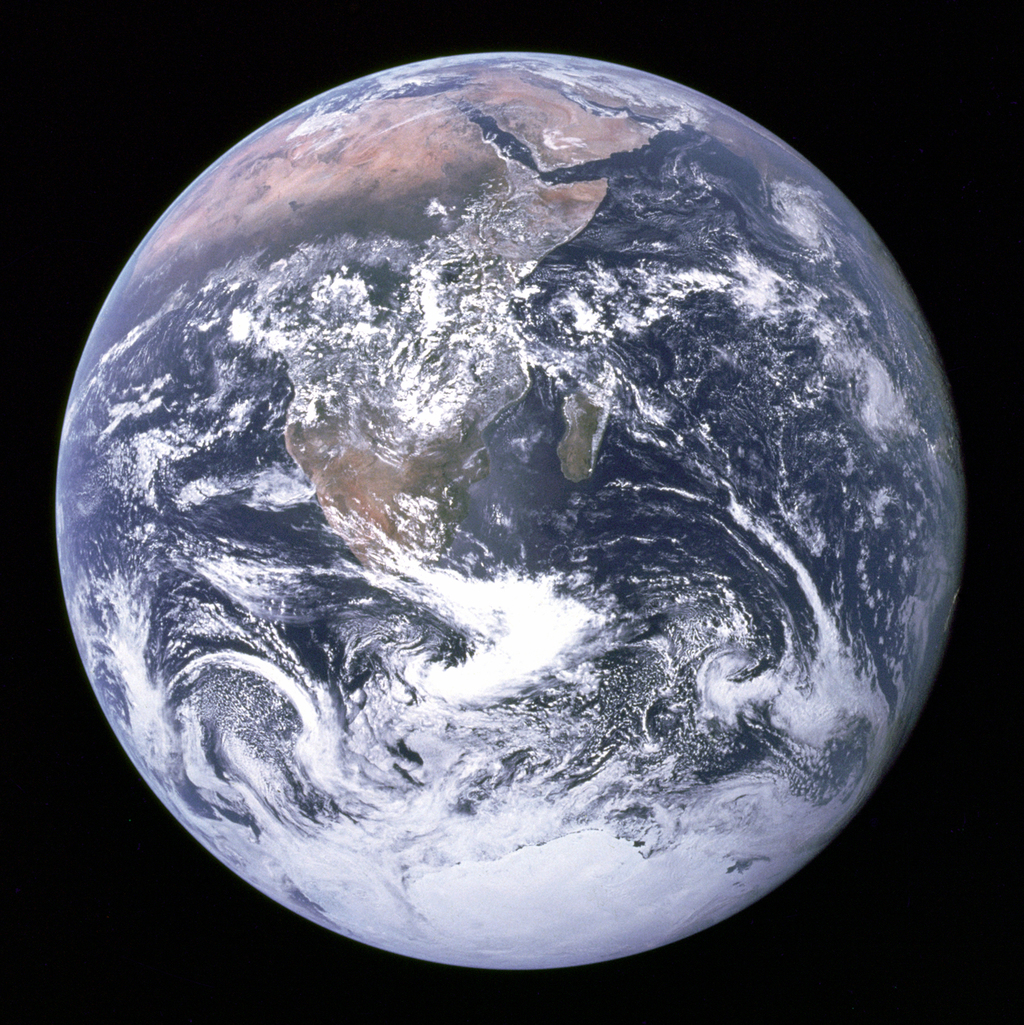
\includegraphics[width=.5\textwidth]{The_Earth_seen_from_Apollo_17}
  \caption{The blue marble photo.}
  \label{fig:bluemarble}
\end{figure}

\section{\LaTeX{}}
This text is no introduction to \LaTeX{}. For more information, see
for example online resources at \citep{TUG}, where a good start is the document
\url{http://ctan.org/pkg/lshort}. Software can be downloaded for Linux
\url{http://www.tug.org/texlive/}, for Mac
\url{http://www.tug.org/mactex/}, and for Windows
\url{http://www.miktex.org}.

To typeset this document on a Linux or Mac system, write
\begin{lstlisting}[language=sh,frame=single]
pdflatex general_en.tex
bibtex general_en
pdflatex general_en.tex
\end{lstlisting}
at a command line prompt to produce file \texttt{general_en.pdf}.

\subsection{How to write requirements}
\lipsum[7]

There is an environment and commands defined to write requirements,
handle requirement numbering, and making it possible to reference
individual requirements. It should look good also when table spans
multiple pages. See source code for generation of the requirement
table below.

\begin{requirements}
  \requirementno\label{req:myreq} & Description & 2\\
  \requirementno & Description & 1\\
  \requirementno & Description & 1\\
  \requirementno & Description & 1\\
  \requirementno & Description & 1\\
  \requirementno & Description & 1\\
  \requirementno & Description & 1\\
  \requirementno & Description & 1\\
  \requirementno & Description & 1\\
  \requirementno\label{req:myreq2} & Description & 2\\
  \requirementno & Description & 1\\
  \requirementno & Description & 1\\
  \requirementno & Description & 1\\
  \requirementno & Description & 1\\
  \requirementno & Description & 1\\
  \requirementno & Description & 1\\
  \requirementno & Description & 1\\
  \requirementno & Description & 1\\
  \requirementno & Description & 1\\
  \requirementno & Description & 1\\
  \requirementno & Description & 1\\
  \requirementno & Description & 1\\
  \requirementno & Description & 1\\
  \requirementno & Description & 1\\
  \requirementno & Description & 1\\
  \requirementno & Description & 1\\
  \requirementno & Description & 1\\
  \requirementno & Description & 1\\
  \requirementno & Description & 1\\
  \requirementno & Description & 1\\
\end{requirements}

Note that requirements~\ref{req:myreq} and~\ref{req:myreq2} has priority 2.

\clearpage
\bibliography{references}

\cleardoublepage
\appendix
\section{First appendix}
\subsection{First subsection of first appendix}
\lipsum[5]

\subsubsection{Subsection in first appendix}
A text

\subsection{Second section in first appendix}
\lipsum[5]
\subsubsection{Subsection in first appendix}
A text

\section{Second appendix}
\subsection{First subsection in second appendix}
\lipsum[5]

\subsubsection{Subsection in second appendix}
A text

\subsection{Second section in second appendix}
\lipsum[5]
\subsubsection{Subsection in second appendix}
A text

\end{document}

%%% Local Variables:
%%% mode: latex
%%% TeX-master: t
%%% End:
